\documentclass[11pt]{article}
\usepackage[textwidth=18.0cm, textheight=23.0cm, top=2.0cm]{geometry}
\usepackage{pst-all}
\usepackage{amssymb}
\usepackage{tikz}
\usepackage{underscore}\begin{document}
\pagestyle{empty}


ClassName: \underline{\textbf{Class_03.2bp-21}}
\par
BinSize: \underline{\textbf{40 × 40}}
\par
ReduceSize: \underline{\textbf{40 × 40}}
\par
TypeNum: \underline{\textbf{58}}
\par
Num: \underline{\textbf{60}}
\par
OutS: \underline{\textbf{20800}}
\par
InS: \underline{\textbf{18220}}
\par
Rate: \underline{\textbf{0.876}}
\par
UB: \underline{\textbf{13}}
\par
LB0: \underline{\textbf{13}}
\par
LB: \underline{\textbf{13}}
\par
LBWithCut: \underline{\textbf{13}}
\par
NodeCut: \underline{\textbf{0}}
\par
ExtendedNodeCnt: \underline{\textbf{1}}
\par
GenNodeCnt: \underline{\textbf{1}}
\par
PrimalNode: \underline{\textbf{0}}
\par
ColumnCount: \underline{\textbf{13}}
\par
TotalCutCount: \underline{\textbf{0}}
\par
RootCutCount: \underline{\textbf{0}}
\par
LPSolverCnt: \underline{\textbf{1}}
\par
PricingSolverCnt: \underline{\textbf{0}}
\par
BranchAndBoundNum: \underline{\textbf{1}}
\par
isOpt: \underline{\textbf{true}}
\par
TimeOnPrimal: \underline{\textbf{0.000 s}}
\par
TimeOnPricing: \underline{\textbf{0.000 s}}
\par
TimeOnRmp: \underline{\textbf{0.063 s}}
\par
TotalTime: \underline{\textbf{0.125 s}}
\par
\newpage


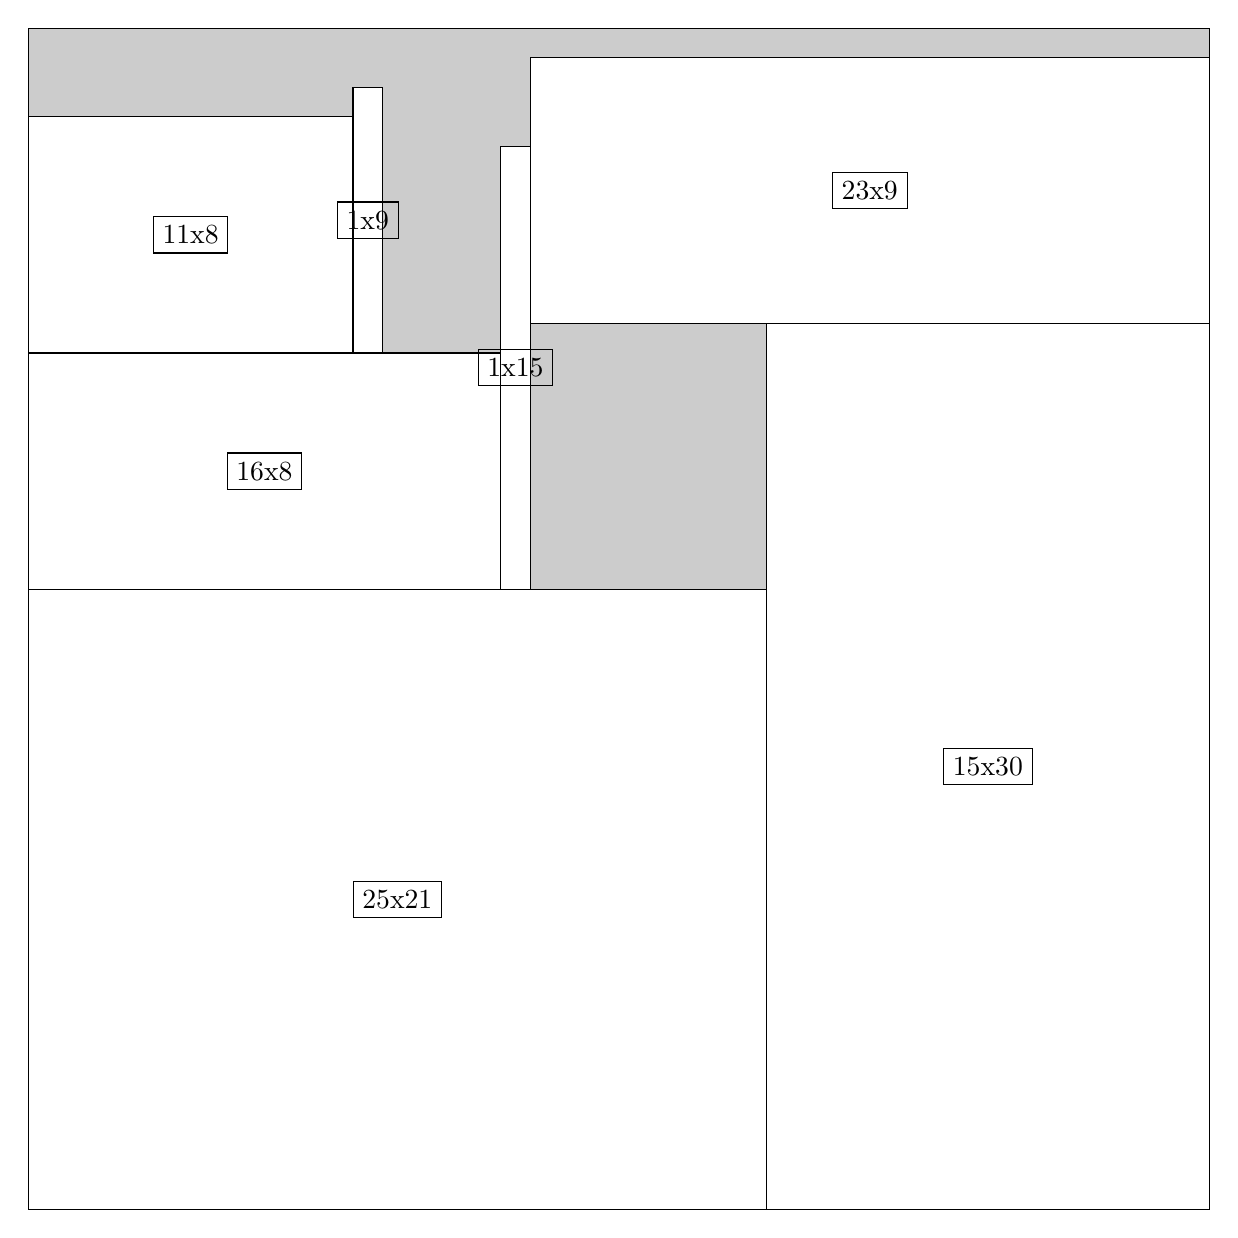
\begin{tikzpicture}[shorten >=1pt,scale=1.0,every node/.style={scale=1.0},->]
\tikzstyle{vertex}=[circle,fill=black!25,minimum size=14pt,inner sep=0pt]
\filldraw[fill=gray!40!white, draw=black] (0,0) rectangle (15.0,15.0);
\foreach \name/\x/\y/\w/\h in {25x21/0.0/0.0/9.375/7.875,15x30/9.375/0.0/5.625/11.25,16x8/0.0/7.875/6.0/3.0,23x9/6.375/11.25/8.625/3.375,11x8/0.0/10.875/4.125/3.0,1x15/6.0/7.875/0.375/5.625,1x9/4.125/10.875/0.375/3.375}
\filldraw[fill=white!40!white, draw=black] (\x,\y) rectangle node[draw] (\name) {\name} ++(\w,\h);
\end{tikzpicture}


w =25 , h =21 , x =0 , y =0 , v =525
\par
w =15 , h =30 , x =25 , y =0 , v =450
\par
w =16 , h =8 , x =0 , y =21 , v =128
\par
w =23 , h =9 , x =17 , y =30 , v =207
\par
w =11 , h =8 , x =0 , y =29 , v =88
\par
w =1 , h =15 , x =16 , y =21 , v =15
\par
w =1 , h =9 , x =11 , y =29 , v =9
\par
\newpage


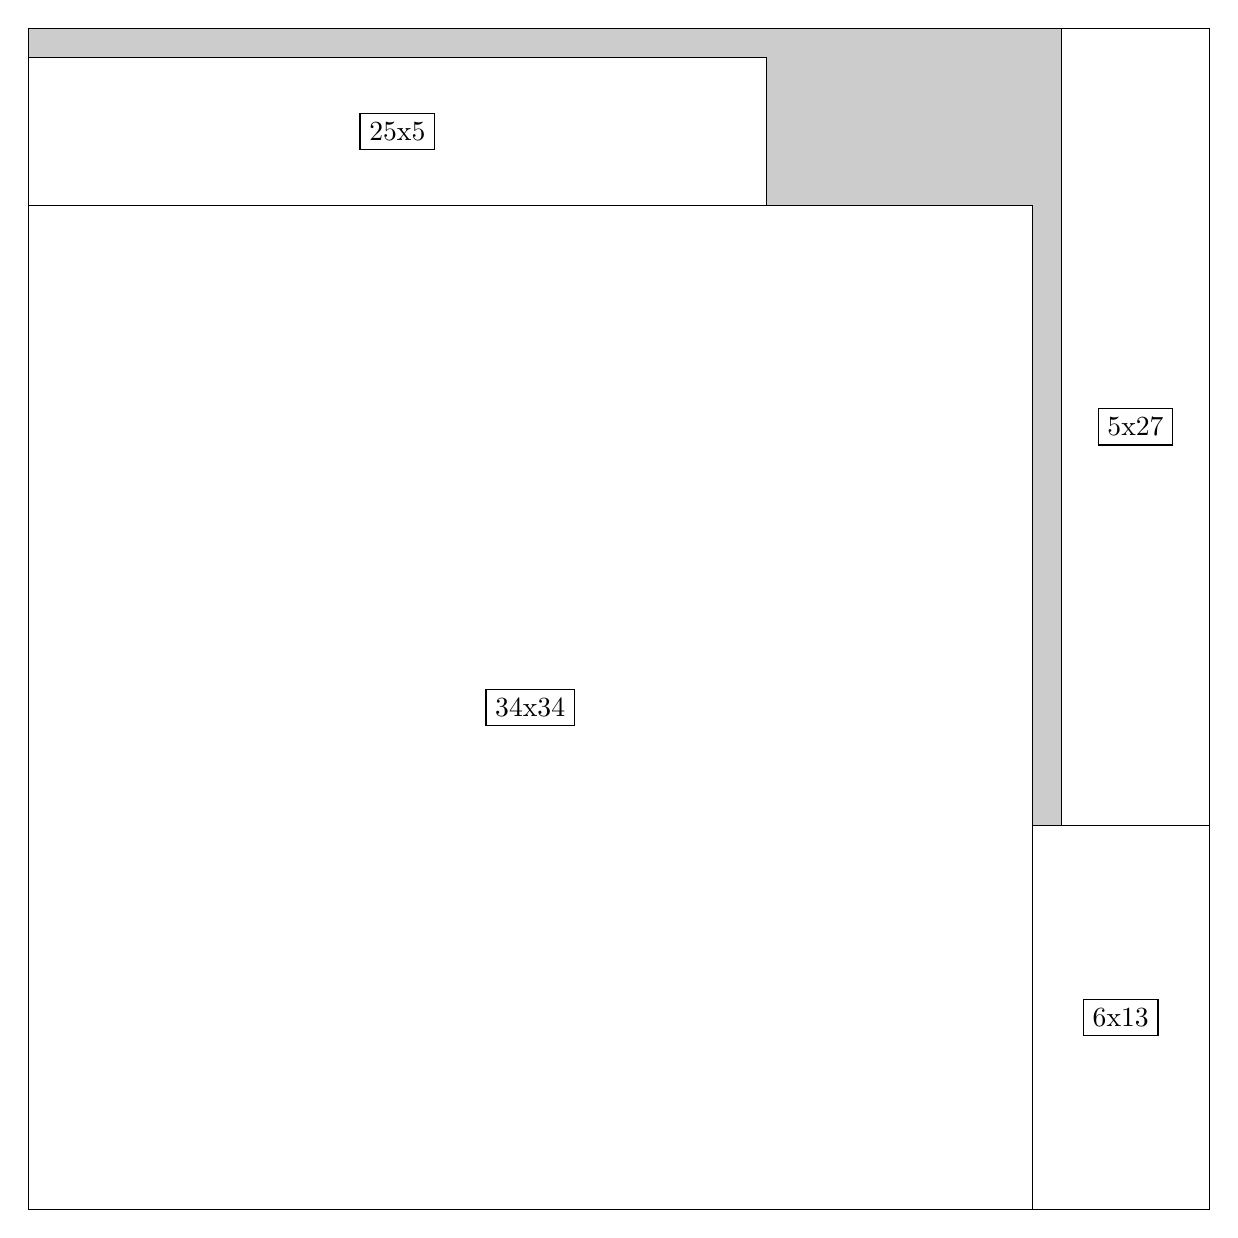
\begin{tikzpicture}[shorten >=1pt,scale=1.0,every node/.style={scale=1.0},->]
\tikzstyle{vertex}=[circle,fill=black!25,minimum size=14pt,inner sep=0pt]
\filldraw[fill=gray!40!white, draw=black] (0,0) rectangle (15.0,15.0);
\foreach \name/\x/\y/\w/\h in {34x34/0.0/0.0/12.75/12.75,25x5/0.0/12.75/9.375/1.875,6x13/12.75/0.0/2.25/4.875,5x27/13.125/4.875/1.875/10.125}
\filldraw[fill=white!40!white, draw=black] (\x,\y) rectangle node[draw] (\name) {\name} ++(\w,\h);
\end{tikzpicture}


w =34 , h =34 , x =0 , y =0 , v =1156
\par
w =25 , h =5 , x =0 , y =34 , v =125
\par
w =6 , h =13 , x =34 , y =0 , v =78
\par
w =5 , h =27 , x =35 , y =13 , v =135
\par
\newpage


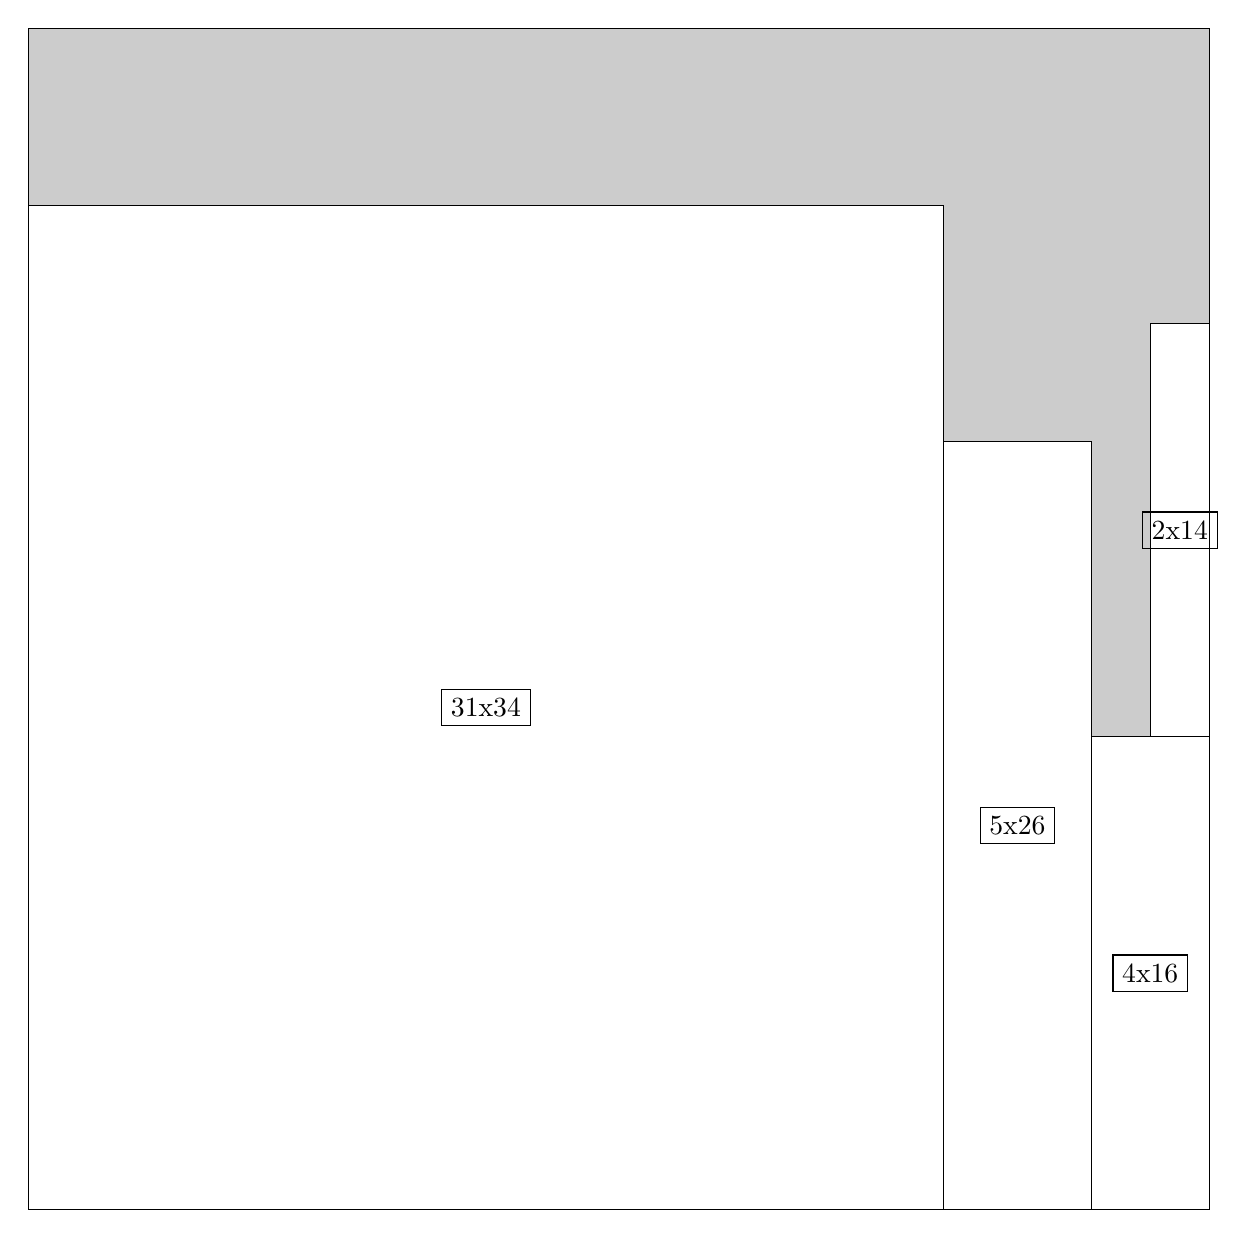
\begin{tikzpicture}[shorten >=1pt,scale=1.0,every node/.style={scale=1.0},->]
\tikzstyle{vertex}=[circle,fill=black!25,minimum size=14pt,inner sep=0pt]
\filldraw[fill=gray!40!white, draw=black] (0,0) rectangle (15.0,15.0);
\foreach \name/\x/\y/\w/\h in {31x34/0.0/0.0/11.625/12.75,5x26/11.625/0.0/1.875/9.75,4x16/13.5/0.0/1.5/6.0,2x14/14.25/6.0/0.75/5.25}
\filldraw[fill=white!40!white, draw=black] (\x,\y) rectangle node[draw] (\name) {\name} ++(\w,\h);
\end{tikzpicture}


w =31 , h =34 , x =0 , y =0 , v =1054
\par
w =5 , h =26 , x =31 , y =0 , v =130
\par
w =4 , h =16 , x =36 , y =0 , v =64
\par
w =2 , h =14 , x =38 , y =16 , v =28
\par
\newpage


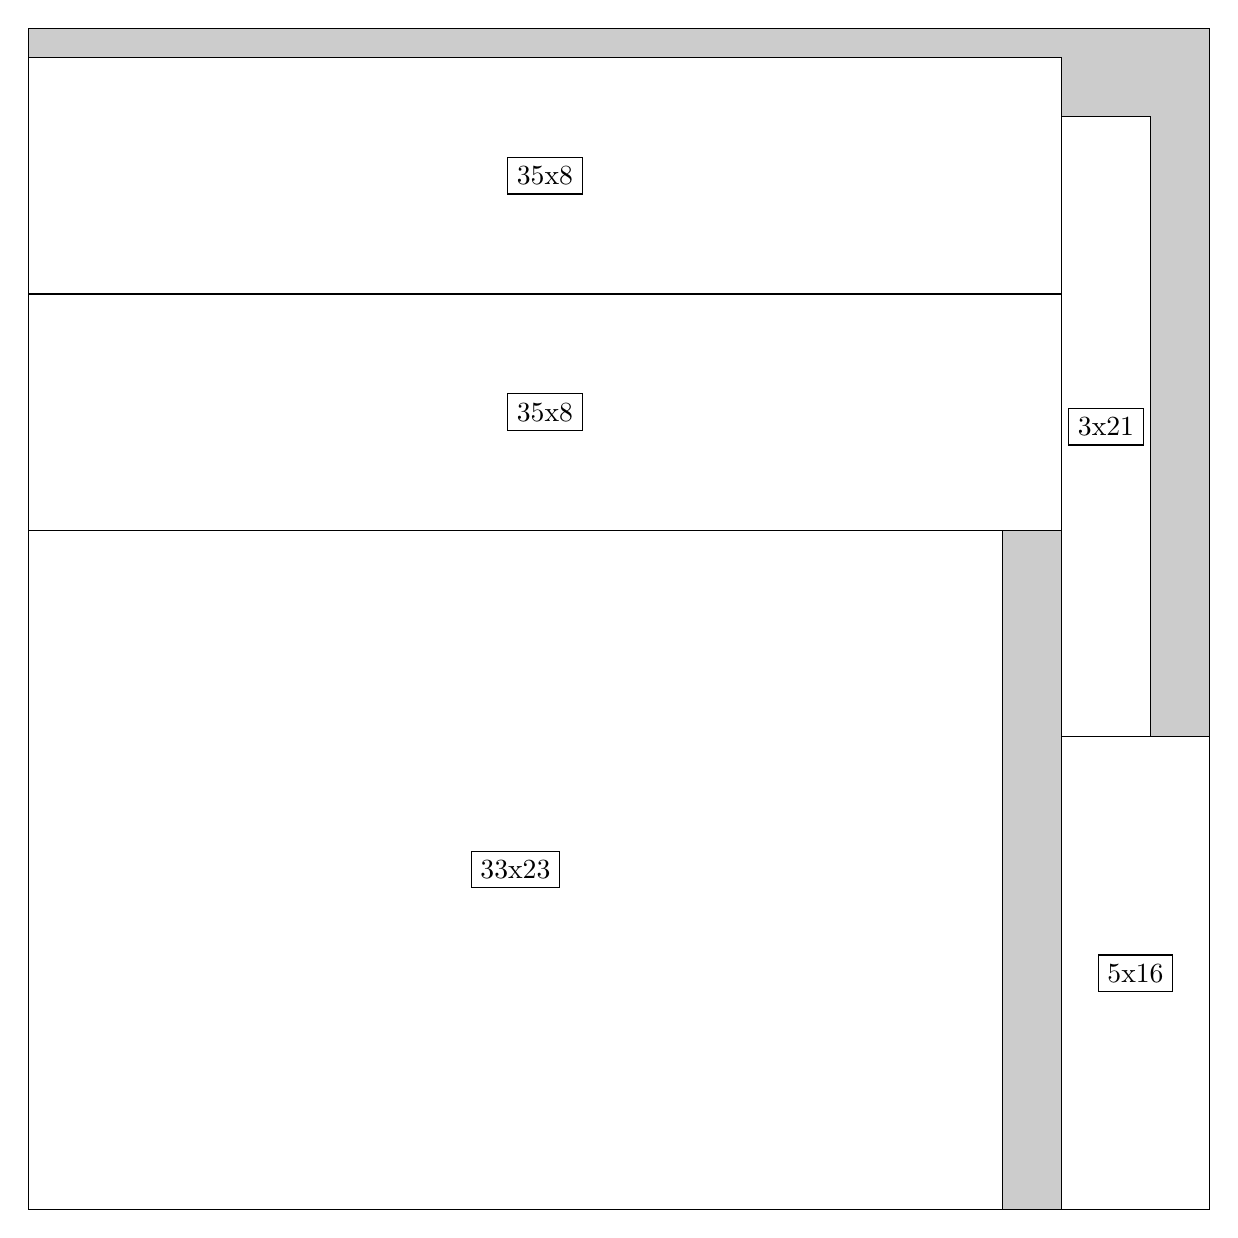
\begin{tikzpicture}[shorten >=1pt,scale=1.0,every node/.style={scale=1.0},->]
\tikzstyle{vertex}=[circle,fill=black!25,minimum size=14pt,inner sep=0pt]
\filldraw[fill=gray!40!white, draw=black] (0,0) rectangle (15.0,15.0);
\foreach \name/\x/\y/\w/\h in {33x23/0.0/0.0/12.375/8.625,35x8/0.0/8.625/13.125/3.0,35x8/0.0/11.625/13.125/3.0,5x16/13.125/0.0/1.875/6.0,3x21/13.125/6.0/1.125/7.875}
\filldraw[fill=white!40!white, draw=black] (\x,\y) rectangle node[draw] (\name) {\name} ++(\w,\h);
\end{tikzpicture}


w =33 , h =23 , x =0 , y =0 , v =759
\par
w =35 , h =8 , x =0 , y =23 , v =280
\par
w =35 , h =8 , x =0 , y =31 , v =280
\par
w =5 , h =16 , x =35 , y =0 , v =80
\par
w =3 , h =21 , x =35 , y =16 , v =63
\par
\newpage


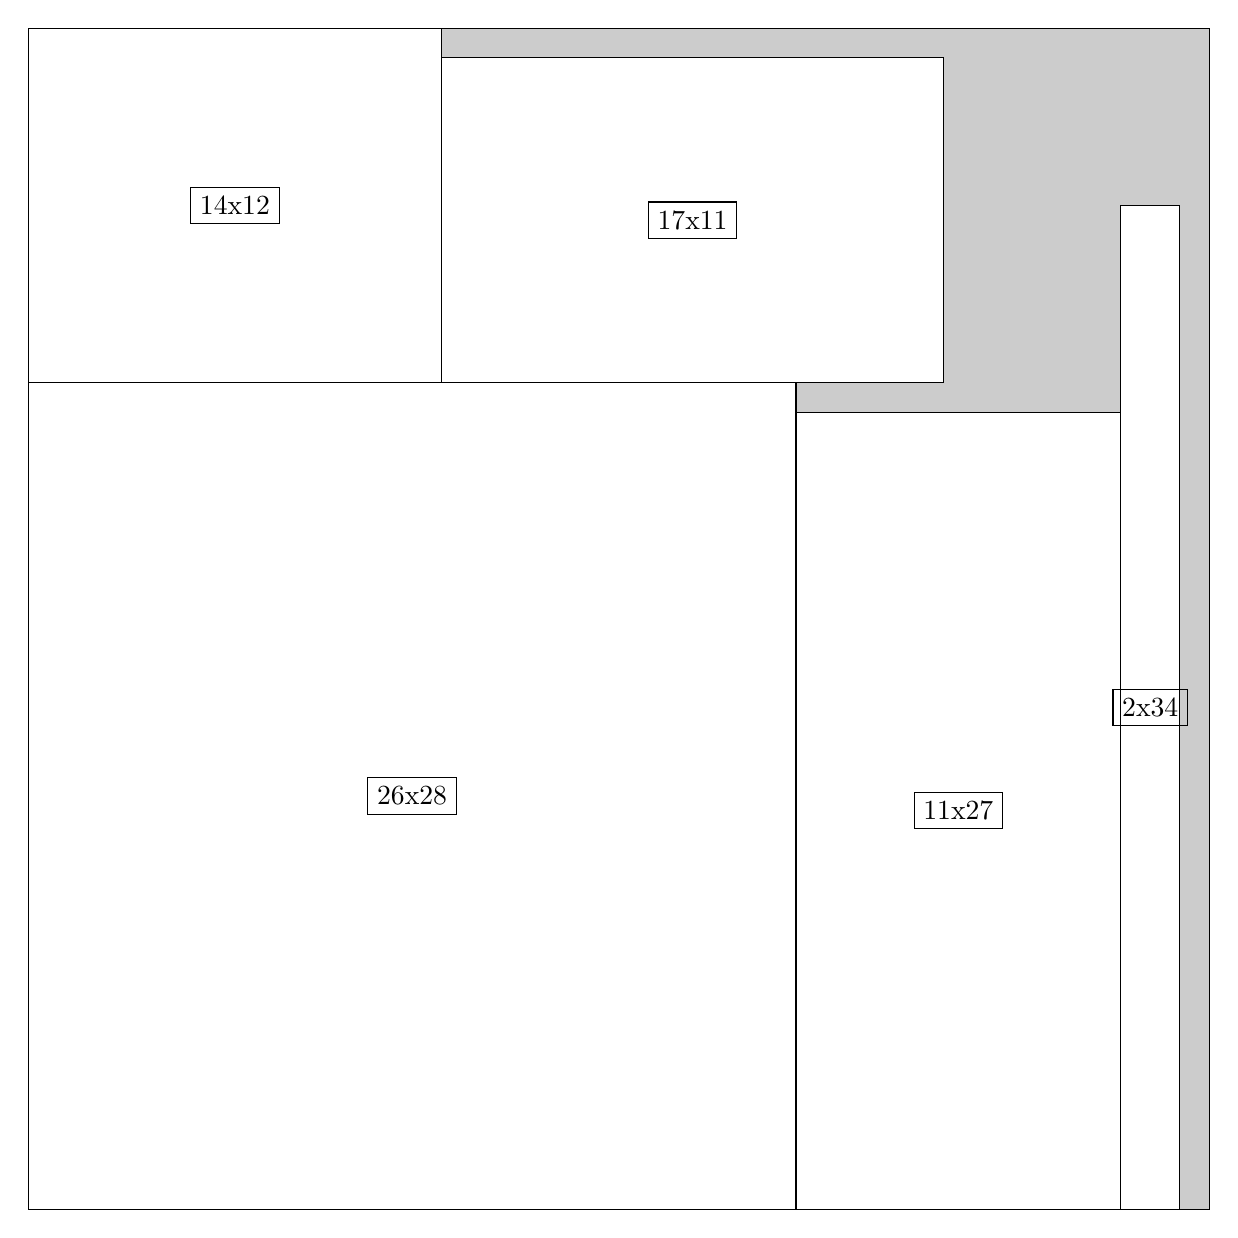
\begin{tikzpicture}[shorten >=1pt,scale=1.0,every node/.style={scale=1.0},->]
\tikzstyle{vertex}=[circle,fill=black!25,minimum size=14pt,inner sep=0pt]
\filldraw[fill=gray!40!white, draw=black] (0,0) rectangle (15.0,15.0);
\foreach \name/\x/\y/\w/\h in {26x28/0.0/0.0/9.75/10.5,11x27/9.75/0.0/4.125/10.125,17x11/5.25/10.5/6.375/4.125,14x12/0.0/10.5/5.25/4.5,2x34/13.875/0.0/0.75/12.75}
\filldraw[fill=white!40!white, draw=black] (\x,\y) rectangle node[draw] (\name) {\name} ++(\w,\h);
\end{tikzpicture}


w =26 , h =28 , x =0 , y =0 , v =728
\par
w =11 , h =27 , x =26 , y =0 , v =297
\par
w =17 , h =11 , x =14 , y =28 , v =187
\par
w =14 , h =12 , x =0 , y =28 , v =168
\par
w =2 , h =34 , x =37 , y =0 , v =68
\par
\newpage


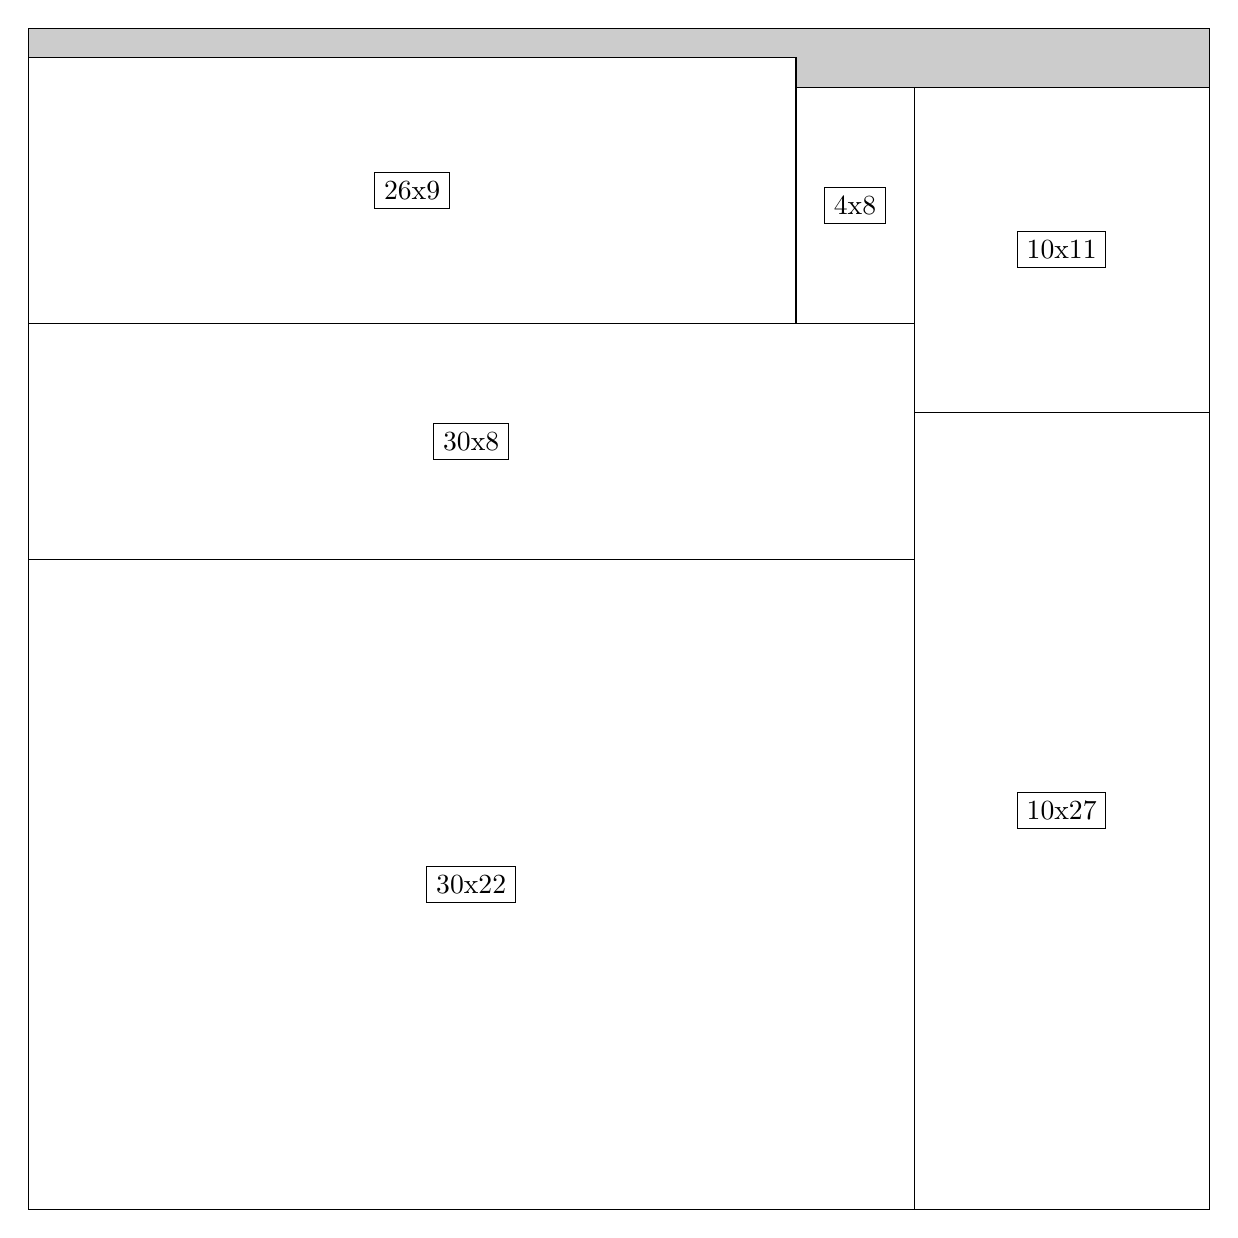
\begin{tikzpicture}[shorten >=1pt,scale=1.0,every node/.style={scale=1.0},->]
\tikzstyle{vertex}=[circle,fill=black!25,minimum size=14pt,inner sep=0pt]
\filldraw[fill=gray!40!white, draw=black] (0,0) rectangle (15.0,15.0);
\foreach \name/\x/\y/\w/\h in {30x22/0.0/0.0/11.25/8.25,10x27/11.25/0.0/3.75/10.125,30x8/0.0/8.25/11.25/3.0,26x9/0.0/11.25/9.75/3.375,10x11/11.25/10.125/3.75/4.125,4x8/9.75/11.25/1.5/3.0}
\filldraw[fill=white!40!white, draw=black] (\x,\y) rectangle node[draw] (\name) {\name} ++(\w,\h);
\end{tikzpicture}


w =30 , h =22 , x =0 , y =0 , v =660
\par
w =10 , h =27 , x =30 , y =0 , v =270
\par
w =30 , h =8 , x =0 , y =22 , v =240
\par
w =26 , h =9 , x =0 , y =30 , v =234
\par
w =10 , h =11 , x =30 , y =27 , v =110
\par
w =4 , h =8 , x =26 , y =30 , v =32
\par
\newpage


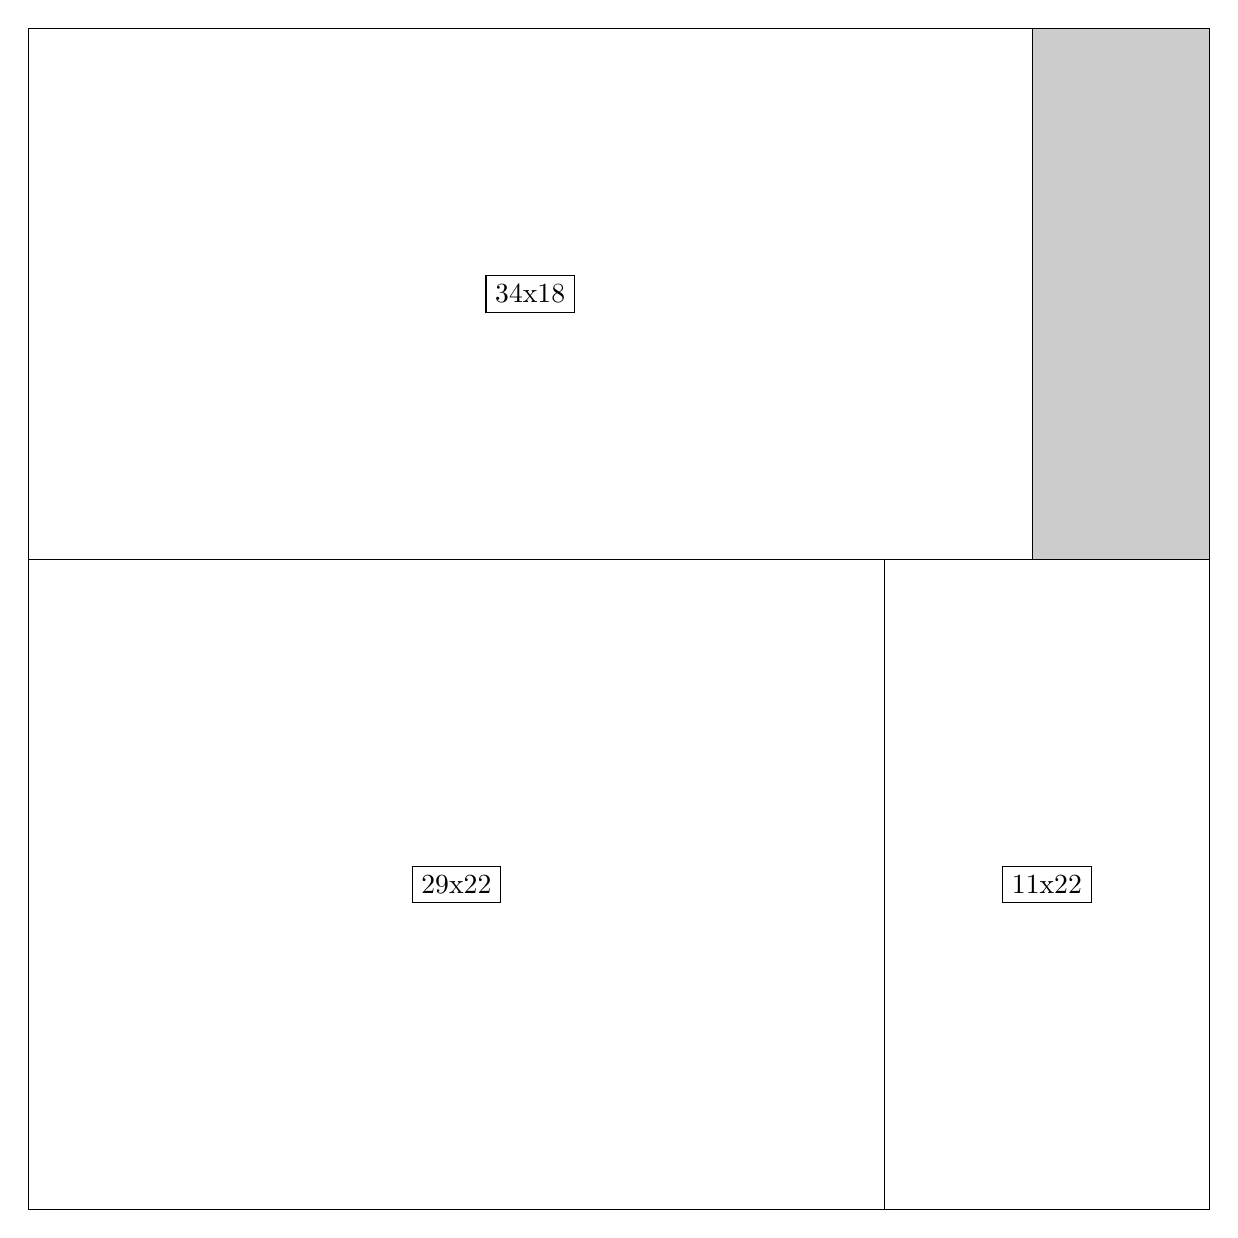
\begin{tikzpicture}[shorten >=1pt,scale=1.0,every node/.style={scale=1.0},->]
\tikzstyle{vertex}=[circle,fill=black!25,minimum size=14pt,inner sep=0pt]
\filldraw[fill=gray!40!white, draw=black] (0,0) rectangle (15.0,15.0);
\foreach \name/\x/\y/\w/\h in {29x22/0.0/0.0/10.875/8.25,34x18/0.0/8.25/12.75/6.75,11x22/10.875/0.0/4.125/8.25}
\filldraw[fill=white!40!white, draw=black] (\x,\y) rectangle node[draw] (\name) {\name} ++(\w,\h);
\end{tikzpicture}


w =29 , h =22 , x =0 , y =0 , v =638
\par
w =34 , h =18 , x =0 , y =22 , v =612
\par
w =11 , h =22 , x =29 , y =0 , v =242
\par
\newpage


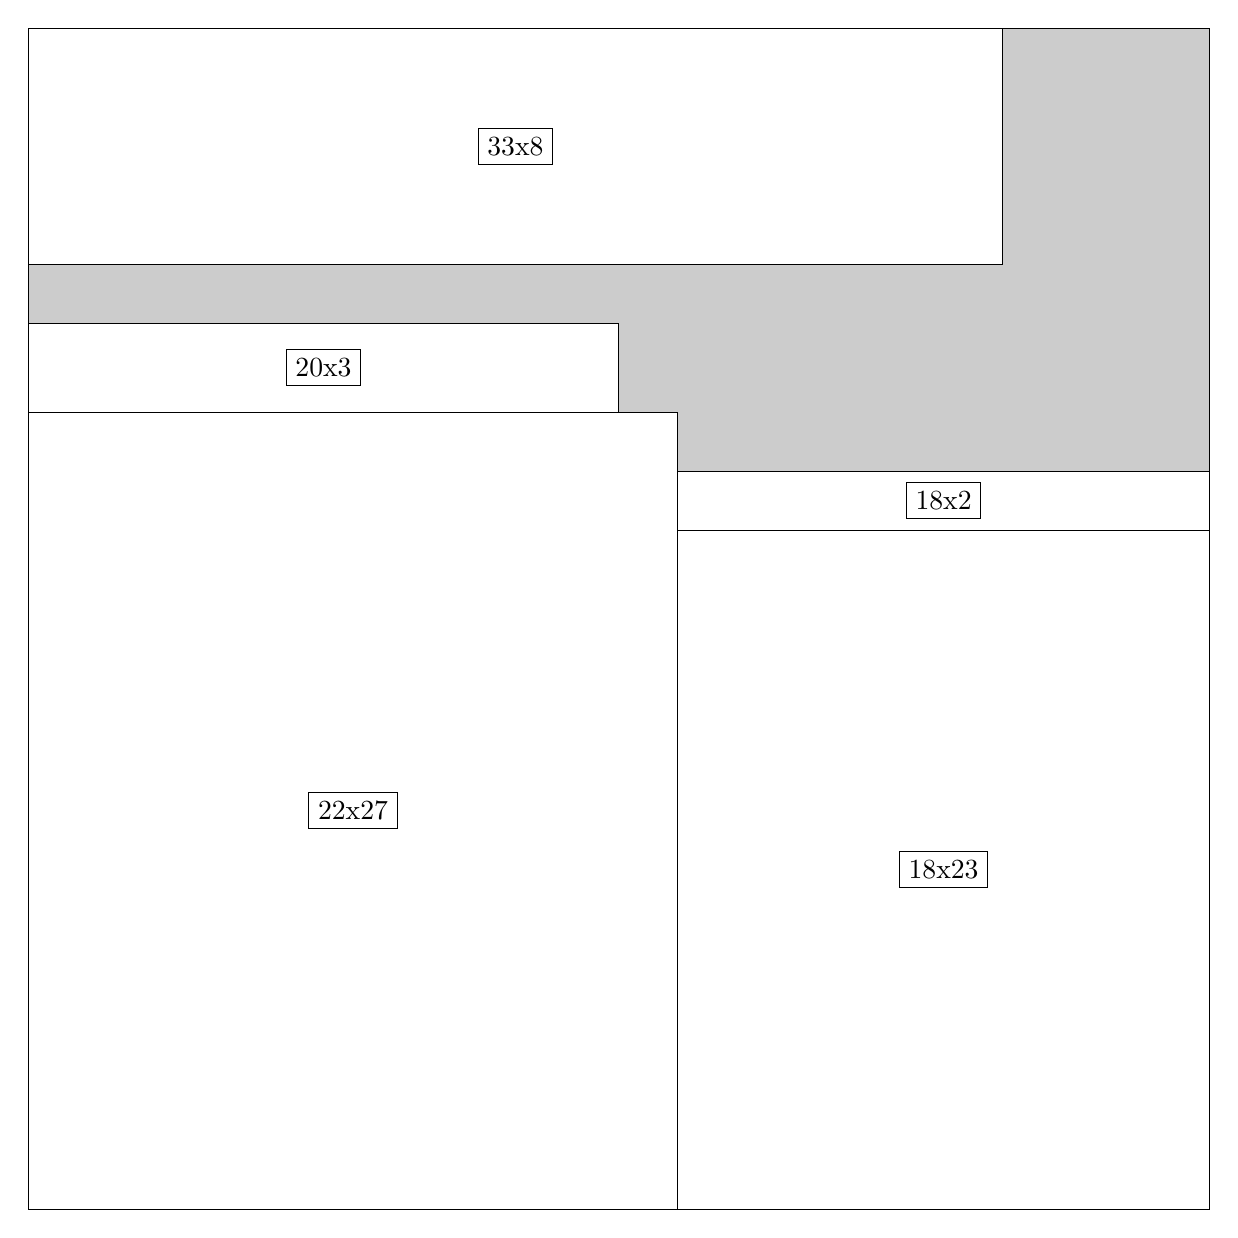
\begin{tikzpicture}[shorten >=1pt,scale=1.0,every node/.style={scale=1.0},->]
\tikzstyle{vertex}=[circle,fill=black!25,minimum size=14pt,inner sep=0pt]
\filldraw[fill=gray!40!white, draw=black] (0,0) rectangle (15.0,15.0);
\foreach \name/\x/\y/\w/\h in {22x27/0.0/0.0/8.25/10.125,18x23/8.25/0.0/6.75/8.625,33x8/0.0/12.0/12.375/3.0,20x3/0.0/10.125/7.5/1.125,18x2/8.25/8.625/6.75/0.75}
\filldraw[fill=white!40!white, draw=black] (\x,\y) rectangle node[draw] (\name) {\name} ++(\w,\h);
\end{tikzpicture}


w =22 , h =27 , x =0 , y =0 , v =594
\par
w =18 , h =23 , x =22 , y =0 , v =414
\par
w =33 , h =8 , x =0 , y =32 , v =264
\par
w =20 , h =3 , x =0 , y =27 , v =60
\par
w =18 , h =2 , x =22 , y =23 , v =36
\par
\newpage


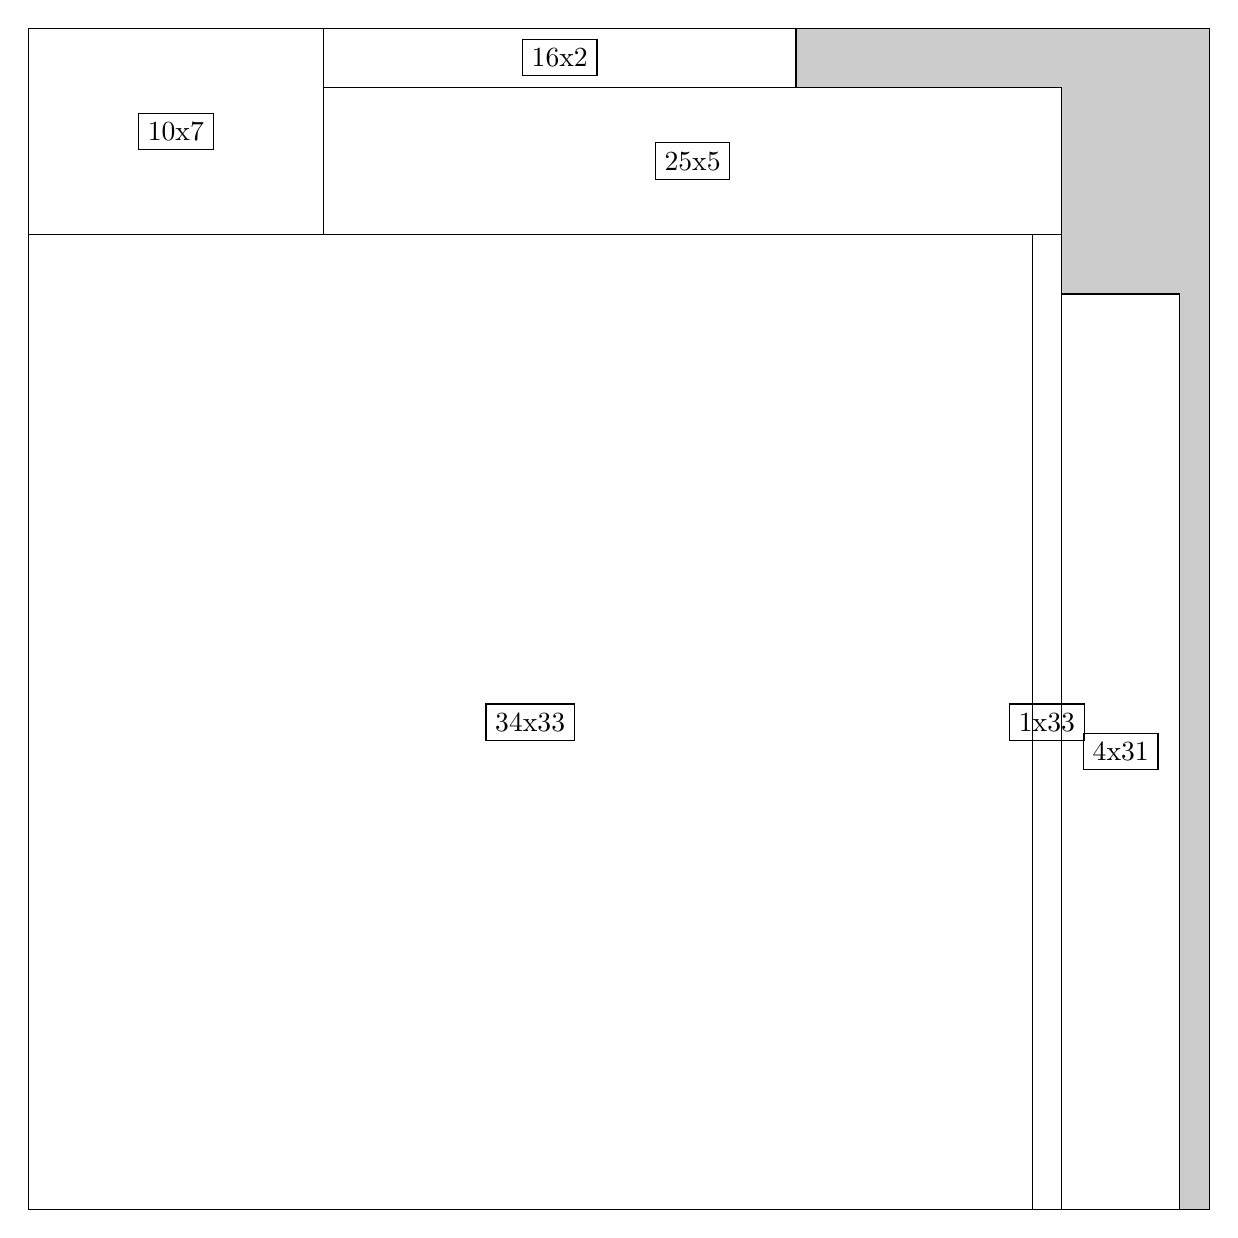
\begin{tikzpicture}[shorten >=1pt,scale=1.0,every node/.style={scale=1.0},->]
\tikzstyle{vertex}=[circle,fill=black!25,minimum size=14pt,inner sep=0pt]
\filldraw[fill=gray!40!white, draw=black] (0,0) rectangle (15.0,15.0);
\foreach \name/\x/\y/\w/\h in {34x33/0.0/0.0/12.75/12.375,10x7/0.0/12.375/3.75/2.625,25x5/3.75/12.375/9.375/1.875,4x31/13.125/0.0/1.5/11.625,1x33/12.75/0.0/0.375/12.375,16x2/3.75/14.25/6.0/0.75}
\filldraw[fill=white!40!white, draw=black] (\x,\y) rectangle node[draw] (\name) {\name} ++(\w,\h);
\end{tikzpicture}


w =34 , h =33 , x =0 , y =0 , v =1122
\par
w =10 , h =7 , x =0 , y =33 , v =70
\par
w =25 , h =5 , x =10 , y =33 , v =125
\par
w =4 , h =31 , x =35 , y =0 , v =124
\par
w =1 , h =33 , x =34 , y =0 , v =33
\par
w =16 , h =2 , x =10 , y =38 , v =32
\par
\newpage


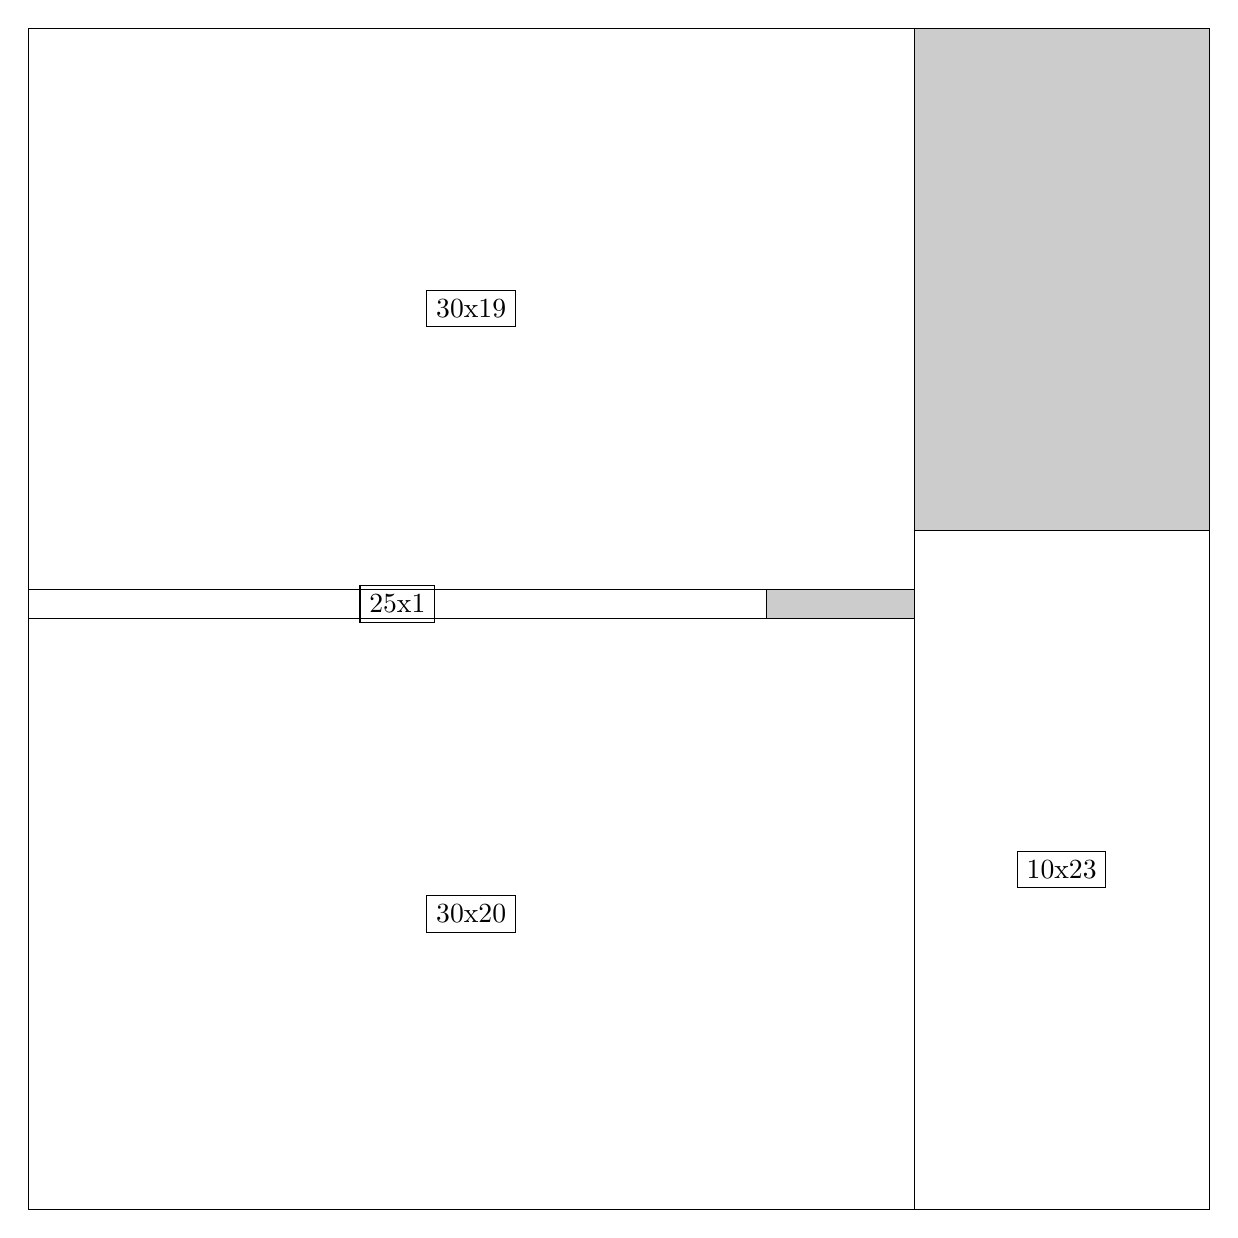
\begin{tikzpicture}[shorten >=1pt,scale=1.0,every node/.style={scale=1.0},->]
\tikzstyle{vertex}=[circle,fill=black!25,minimum size=14pt,inner sep=0pt]
\filldraw[fill=gray!40!white, draw=black] (0,0) rectangle (15.0,15.0);
\foreach \name/\x/\y/\w/\h in {30x20/0.0/0.0/11.25/7.5,30x19/0.0/7.875/11.25/7.125,10x23/11.25/0.0/3.75/8.625,25x1/0.0/7.5/9.375/0.375}
\filldraw[fill=white!40!white, draw=black] (\x,\y) rectangle node[draw] (\name) {\name} ++(\w,\h);
\end{tikzpicture}


w =30 , h =20 , x =0 , y =0 , v =600
\par
w =30 , h =19 , x =0 , y =21 , v =570
\par
w =10 , h =23 , x =30 , y =0 , v =230
\par
w =25 , h =1 , x =0 , y =20 , v =25
\par
\newpage


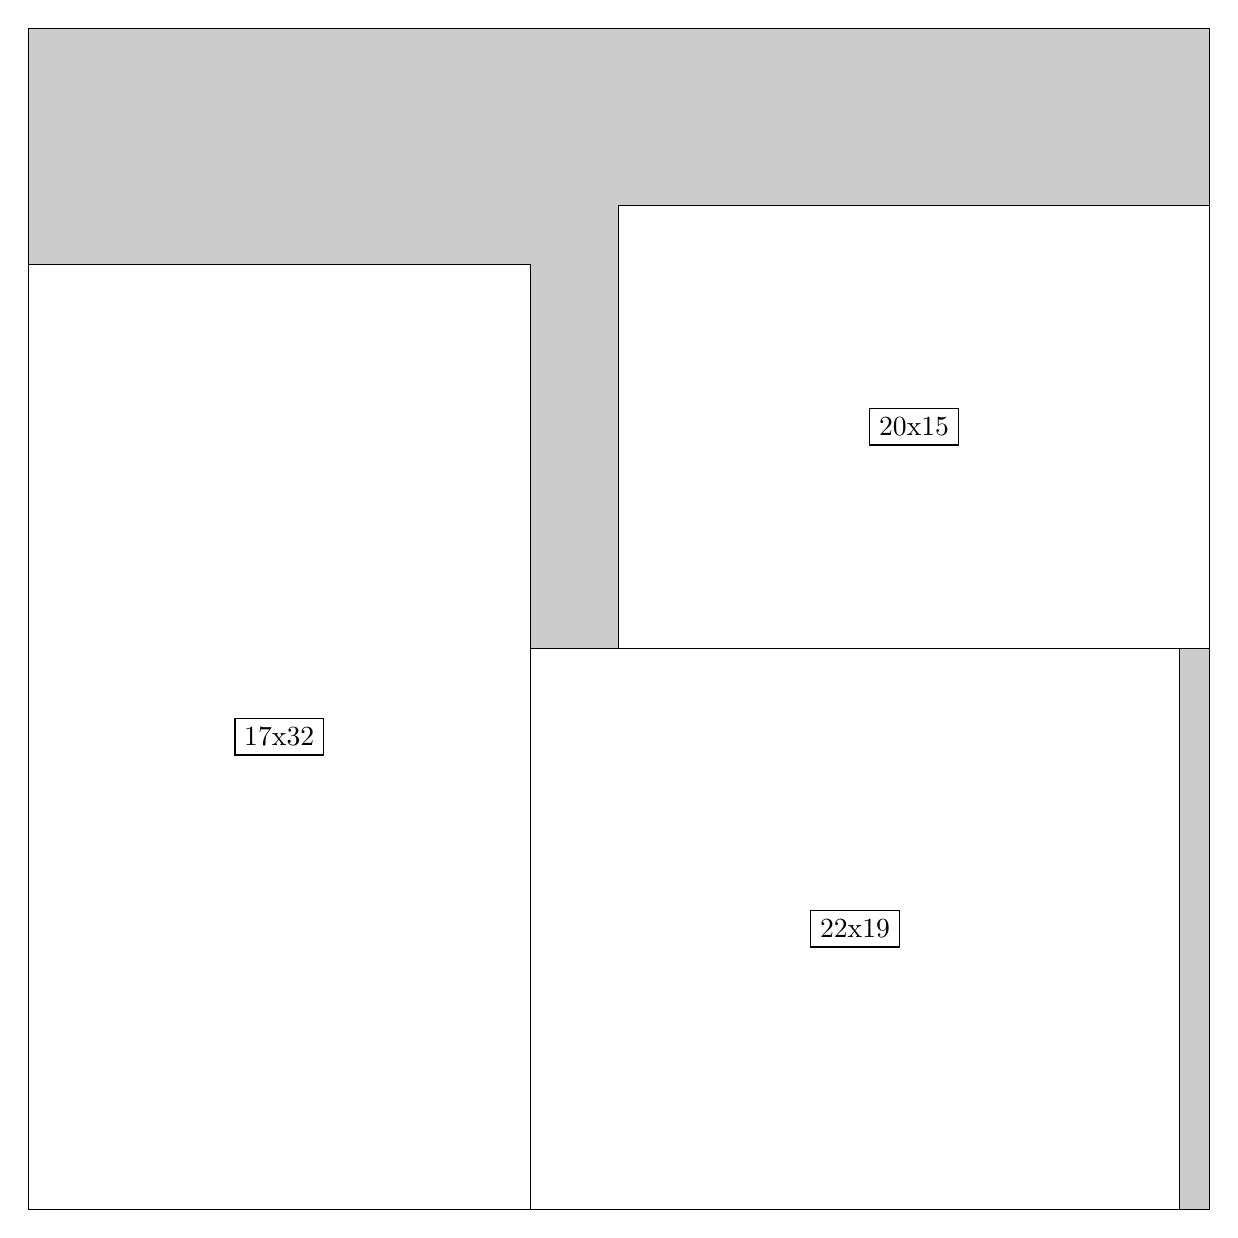
\begin{tikzpicture}[shorten >=1pt,scale=1.0,every node/.style={scale=1.0},->]
\tikzstyle{vertex}=[circle,fill=black!25,minimum size=14pt,inner sep=0pt]
\filldraw[fill=gray!40!white, draw=black] (0,0) rectangle (15.0,15.0);
\foreach \name/\x/\y/\w/\h in {17x32/0.0/0.0/6.375/12.0,22x19/6.375/0.0/8.25/7.125,20x15/7.5/7.125/7.5/5.625}
\filldraw[fill=white!40!white, draw=black] (\x,\y) rectangle node[draw] (\name) {\name} ++(\w,\h);
\end{tikzpicture}


w =17 , h =32 , x =0 , y =0 , v =544
\par
w =22 , h =19 , x =17 , y =0 , v =418
\par
w =20 , h =15 , x =20 , y =19 , v =300
\par
\newpage


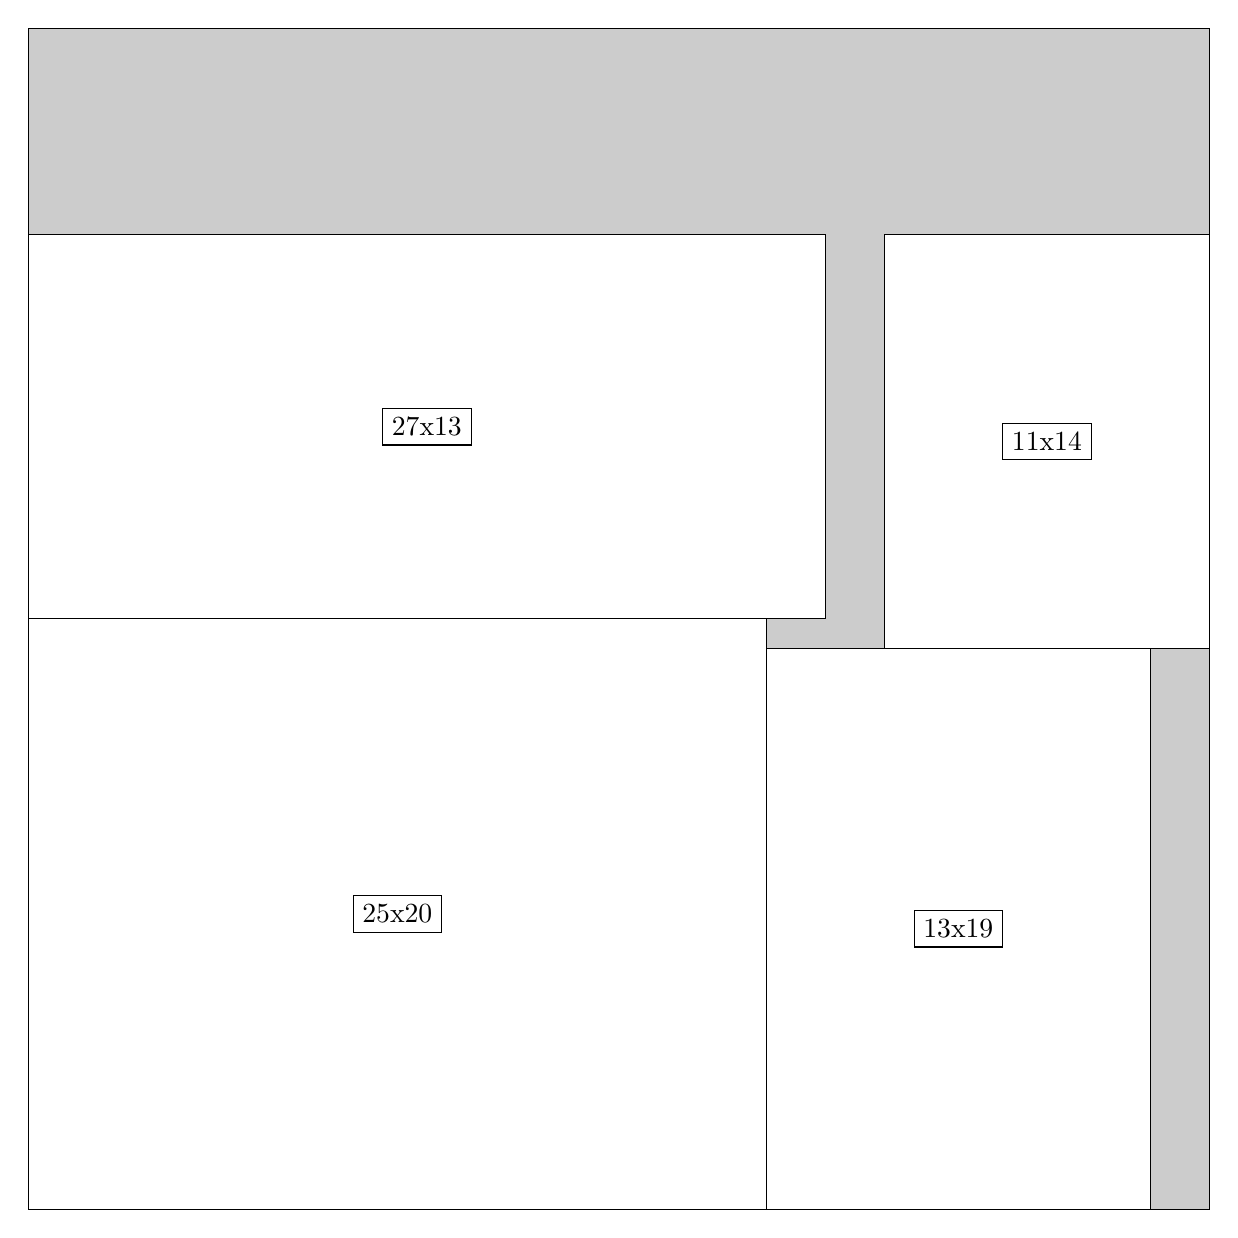
\begin{tikzpicture}[shorten >=1pt,scale=1.0,every node/.style={scale=1.0},->]
\tikzstyle{vertex}=[circle,fill=black!25,minimum size=14pt,inner sep=0pt]
\filldraw[fill=gray!40!white, draw=black] (0,0) rectangle (15.0,15.0);
\foreach \name/\x/\y/\w/\h in {25x20/0.0/0.0/9.375/7.5,27x13/0.0/7.5/10.125/4.875,13x19/9.375/0.0/4.875/7.125,11x14/10.875/7.125/4.125/5.25}
\filldraw[fill=white!40!white, draw=black] (\x,\y) rectangle node[draw] (\name) {\name} ++(\w,\h);
\end{tikzpicture}


w =25 , h =20 , x =0 , y =0 , v =500
\par
w =27 , h =13 , x =0 , y =20 , v =351
\par
w =13 , h =19 , x =25 , y =0 , v =247
\par
w =11 , h =14 , x =29 , y =19 , v =154
\par
\newpage


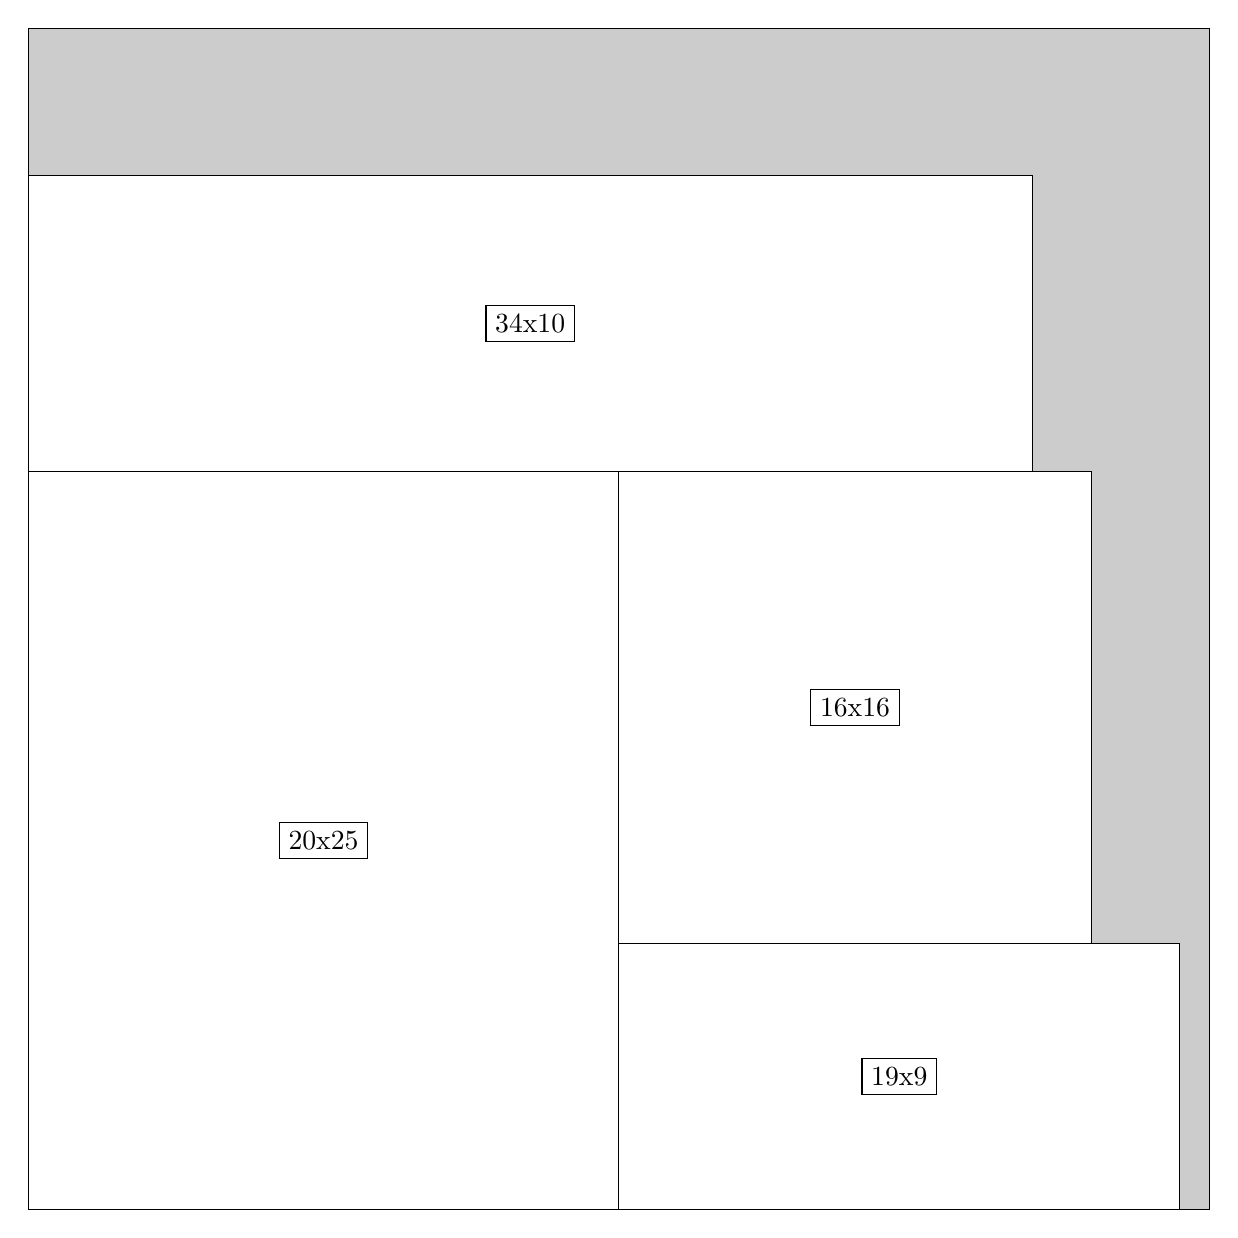
\begin{tikzpicture}[shorten >=1pt,scale=1.0,every node/.style={scale=1.0},->]
\tikzstyle{vertex}=[circle,fill=black!25,minimum size=14pt,inner sep=0pt]
\filldraw[fill=gray!40!white, draw=black] (0,0) rectangle (15.0,15.0);
\foreach \name/\x/\y/\w/\h in {20x25/0.0/0.0/7.5/9.375,34x10/0.0/9.375/12.75/3.75,16x16/7.5/3.375/6.0/6.0,19x9/7.5/0.0/7.125/3.375}
\filldraw[fill=white!40!white, draw=black] (\x,\y) rectangle node[draw] (\name) {\name} ++(\w,\h);
\end{tikzpicture}


w =20 , h =25 , x =0 , y =0 , v =500
\par
w =34 , h =10 , x =0 , y =25 , v =340
\par
w =16 , h =16 , x =20 , y =9 , v =256
\par
w =19 , h =9 , x =20 , y =0 , v =171
\par
\newpage


\end{document}